\documentclass[pdftex,a4paper]{article}
 %% PACKAGES
 \usepackage[dutch]{babel}
 \usepackage{vubtitlepage}
 \usepackage{fancyhdr}
 \usepackage{graphicx}
 \usepackage[utf8]{inputenc}
 \usepackage[T1]{fontenc}
 \usepackage[usenames]{color}
 \usepackage[pdftex,pdfpagelabels]{hyperref}
 \usepackage{amssymb}

 %% CUSTOM COLORS
 \definecolor{grey}{rgb}{0.1804, 0.2039, 0.2118}
 \newcommand{\red}[1]{{\color{red}{#1}}} % rood

 %% CUSTOM COMMANDS
 \newcommand{\tildefix}{\textasciitilde} % ASCII tilde
 \newcommand{\hreftt}[2]{\href{#1}{\color{blue}\texttt{#2}}} % teletype link: URL, title
 \newcommand{\link}[1]{\href{#1}{#1}} % URL
 \newcommand{\linktt}[1]{\hreftt{#1}{\color{blue}#1}} % URL in teletype

 \newcommand{\rotateboxx}[2]{\ifpdf \rotatebox{#1}{#2} \else #2 \fi}
 \newcommand{\sectionInv}[1]{\addcontentsline{toc}{section}{#1}} % invisible section
 \newcommand{\sectionUnN}[1]{\section*{#1}\sectionInv{#1}} % unnumbered section
 \newcommand{\tbd}[1]{{\color{red}{#1}}} % tbd: to be done
 \newcommand{\conj}[1]{#1^{\star}}
 \newcommand{\norm}[1]{\left| #1 \right|}

 %% CUSTOM ENVIRONMENTS
 \newenvironment{quotationgr}{\begin{quotation}\color{grey}}{\end{quotation}}

 %% DOCUMENT PROPERTIES
 \faculty{Faculteit Ingenieurswetenschappen}

 \title{Design van een hoogfrequente versterker en antenne}
 \reason{Hoogfrequente elektronica en antennes}
 \author{\href{mailto:Bert.Follon@vub.ac.be}{Bert Follon},
         \href{mailto:Egon.Geerardyn@vub.ac.be}{Egon Geerardyn}}
 \newcommand{\datum}{\today}
 \date{\datum}
 \hypersetup{colorlinks,%
            citecolor=black,%
            filecolor=black,%
            linkcolor=black,%
            urlcolor=blue,%
            pdfauthor={Egon Geerardyn, Bert Follon},%
            pdftitle={Design van een hoogfrequente versterker en antenne},%
            plainpages=false}
  \pdfpagewidth=\paperwidth
  \pdfpageheight=\paperheight

  


 %% HEADER CONFIG
 \pagestyle{fancy}
  \rhead{\datum}
  \chead{}
  \lhead{HFE: versterker en antenne}
  \cfoot{\thepage}


\begin{document}
  \maketitlepage
  \newpage
  \tableofcontents
  \listoffigures
  \listoftables
  De broncode en een digitale versie van het verslag zijn beschikbaar op \cite{github}.
  \newpage
  \part{Versterker}
  \label{sec:Amp}
    
    % VERSTERKER

    In dit verslag wordt het designproces van hoogfrequente single-stage
    versterker besproken die gerealiseerd wordt in common emitter-opstelling.

    Hierbij is de gebruikte NPN-transistor een BFR91A en werd
    het werkingspunt in \cite{lesWendy} gespecificeerd zoals weergegeven in
    \autoref{tbl:OPSpec}.
      \begin{table}[h!]
        \begin{center}

        \caption{DC werkingspunt transistor}
        \label{tbl:OPSpec}
        
 \begin{tabular}{|l|l|l|l|} 
\hline \textbf{Groep} & \textbf{Frequentie $f_0$} & \textbf{$V_{ce}$} & \textbf{$I_c$}\\ 
\hline $1$ & $1445$ MHz & $5$ V & $5$ mA \\ 
\hline \end{tabular} 

        \end{center}
      \end{table} 
    
    Voor deze werkingsfrequentie werden de $S$-parameters gegeven in \cite{lesWendy}:
    \[
S = \left[ \begin{array}{cc} 
S_{11} & S_{12} \\ 
 S_{21} & S_{22} \\ 
\end{array} \right] 
 \approx \left[ \begin{array}{cc} 
-0.104 +0.181 j & 0.102 +0.154 j \\ 
1.369 +1.397 j & 0.355 -0.318 j \\ 
\end{array} \right] \label{eq:S}
\]
    
\section{Stabiliteit}
    We controleren de nodige en voldoende voorwaarde voor stabiliteit van de versterker
    door middel van formules 11.71 en 11.72 van \cite{Pozar}.
    Dit is het Rollet-stabiliteitscriterium.
    \[
      K = \frac{1 - \left| S_{11} \right|^2 - \left| S_{22} \right|^2 + \left| \Delta \right|^2}{2 \left| S_{12}S_{21} \right|} > 1
    \]
    \[
      \left| \Delta \right| < 1
    \]
    \[
      \Delta = \det{S} = S_{11}S_{22} - S_{12}S_{21}
    \]
    Numeriek geeft dit:
    \[
K \approx 1.113 \qquad \qquad 
|\Delta| \approx |0.096 -0.256j| \approx 0.273 
\]

    Aan de stabiliteitsvoorwaarden is voldaan, zodat men kan besluiten dat de te
    realiseren versterker onconditioneel stabiel is.
  \section{Stabiliteitscirkels}
    Vermits de versterker onconditioneel stabiel is, zullen de stabiliteitscirkels
    ofwel de volledige Smith Chart omvatten ofwel buiten de Smith Chart vallen.
    Toch wordt dit nogmaals gecontroleerd.

    De stabiliteitscirkels geven de reflectiefactoren (en dus ook de matching-
    impedanties) aan waarvoor de hele schakeling nog net stabiel is voor de
    opgegeven werkingsfrequentie. Onvoorwaardelijke stabiliteit zegt dus enkel
    dat indien de versterker voorzien wordt van passieve netwerken aan de in-
    en uitgang dat er geen oscillator op de werkingsfrequentie gemaakt is.
    Wat echter niet aangetoond wordt met dit stabiliteitscriterium is de
    afwezigheid van oscillaties op andere frequenties!
    
    Met formules 11.68 en 11.69 uit \cite{Pozar}, worden middelpunt $C$ en
    straal $R$ van de stabiliteitscirkels bepaald.
    \[
      C_L = \frac{\conj{\left(S_{22} - \Delta \conj{S_{11}}\right)}}{\left| S_{22} \right|^2 - \left|\Delta\right|^2}
      \qquad \qquad \qquad
      R_L = \left| \frac{S_{12}S_{21}}{\left| S_{22} \right|^2 - \left|\Delta\right|^2}\right|
    \]
    \[
      C_S = \frac{\conj{\left(S_{11} - \Delta \conj{S_{22}}\right)}}{\left| S_{11} \right|^2 - \left|\Delta\right|^2}
      \qquad \qquad \qquad
      R_S = \left| \frac{S_{12}S_{21}}{\left| S_{11} \right|^2 - \left|\Delta\right|^2}\right|
    \]
    Dit geeft aanleiding tot volgende waarden:
    \[
	C_L =	  2.70 + j   2.15\qquad \qquad \qquad  	R_L =	  2.37
\]

    \[
	C_S =	  7.04  +7.73 j\qquad \qquad \qquad	R_S =	 11.58
\]

    Op \autoref{fig:stabCirkels} kunnen deze cirkels ge\"inspecteerd worden.
    \begin{figure}[!h]
      \centering
      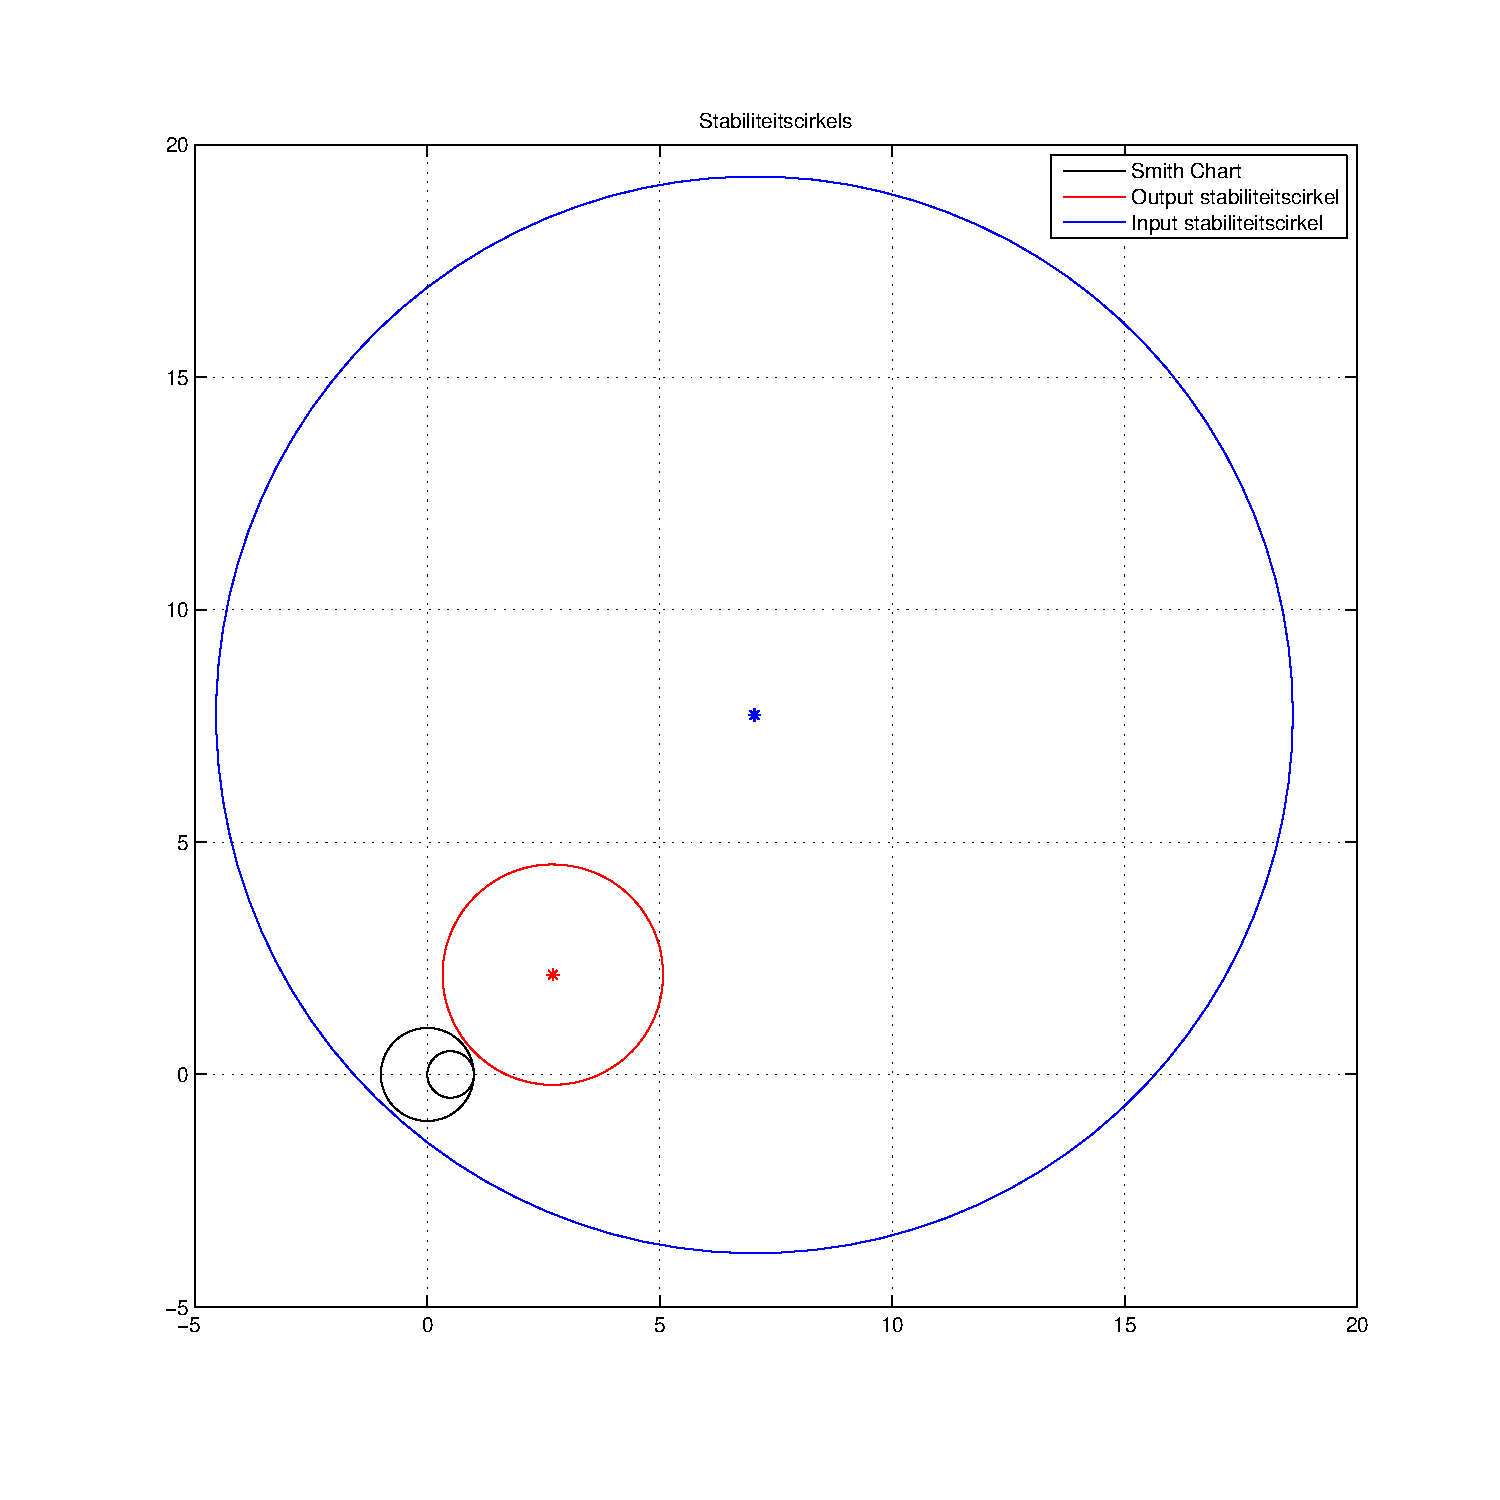
\includegraphics[width=\textwidth,keepaspectratio=true]{fig/stabiliteitscirkels.pdf}  
      \caption{Stabiliteitscirkels} 
      \label{fig:stabCirkels}
    \end{figure}
    Als extra controle, bekijken we welke zones van de Smith Chart stabiel zijn voor input en output. We volgen hier
    een analoge redenering als beschreven op pagina 614 van \cite{Pozar}.
    
    \paragraph{Voor de input} weten we dat indien de output perfect gematcht is
    ($Z_L = Z_0$ en dus ook $\Gamma_L = 0$, oftewel in het midden van de Smith
    Chart), we formule 11.62a uit \cite{Pozar}
    \[
      \left| \Gamma_{in} \right| = \left| S_{11} + \frac{S_{12}S_{21}\Gamma_L}{1 - S_{22}\Gamma_L} \right| < 1
    \]
    kunnen vereenvoudigen tot:
    \[
      \left| S_{11} \right|  < 1
    \]
    als voorwaarde voor stabiliteit. Hieraan is voldaan zoals we kunnen zien uit
    de S-parameters van de transistor. Hierdoor weten we dat het gebied binnen
    de blauwe inputsstabiliteitcirkel stabiel is.
    
    \paragraph{Voor de output} volgt analoog dat indien de input perfect
    gematcht is ($Z_S = Z_0$ en dus ook $\Gamma_S = 0$, oftewel in het
    midden van de Smith Chart), we formule 11.62b uit \cite{Pozar}
    \[
      \left| \Gamma_{out} \right| = \left| S_{22} + \frac{S_{12}S_{21}\Gamma_S}{1 - S_{11}\Gamma_S} \right| < 1
    \]
    kunnen vereenvoudigen tot:
    \[
      \left| S_{22} \right|  < 1
    \]
    als voorwaarde voor stabiliteit. Hieraan is voldaan zoals we kunnen zien uit
    de S-parameters van de transistor. Hierdoor weten we dat het gebied buiten
    de rode outputsstabiliteitcirkel stabiel is.
    

\section{Gebruik van de unilaterale benadering}
  Als verantwoording voor de unilaterale benadering, gebruiken we formule 11.86
  uit \cite{Pozar} die slechts enkele tienden van een dB afwijking mag geven.
  We nemen hiervoor de grenswaarde van $0.8 dB$
  \[
    -0.8 dB < \frac{1}{\left( 1 + U\right)^ 2} < \frac{G_T}{G_{TU}} < \frac{1}{\left( 1 - U\right)^ 2} < 0.8 dB
  \]
  In deze formule is $U$ de \textit{unilateral figure of merit}:
  \[
    U = \frac{\norm{S_{12}} \norm{S_{21}} \norm{S_{11}} \norm{S_{22}}}{ \left( 1 - \norm{S_{11}}^2 \right) \left( 1 - \norm{S_{22}}^2 \right)}
  \]
  In numerieke waarden, geven deze vergelijkingen dus:
    \[
	U \approx	0.04863
\]
\[
-0.8 \,dB < 0.90940 < \frac{G_T}{G_{TU}} < 1.10484 < 0.8 \,dB
\]
\[
-0.8 dB < -0.825 \,dB< \frac{G_T}{G_{TU}} < 0.866 \,dB< 0.8 \,dB
\]

  Vermits deze ongelijkheden geldig zijn, mag de unilaterale benadering gebruikt
  worden.
  
  

\section{Berekening van maximale versterking}
  Aan de hand van \cite{Pozar} en \cite{Gonzalez} wordt de maximale transducergain
  op de gegeven werkingsfrequentie bepaald.
  
  In appendix E van \cite{Gonzalez} werd bewezen dat bovenstaande uitdrukking
  voor een onconditioneel stabiele transistor (K > 1) en simultane input- en
  outputmatching, de maximale versterking uitgedukt
  kan worden als:
  \[
    G_{Tmax} = \frac{\norm{S_{21}}}{\norm{S_{12}}} \left( K - \sqrt{K^2-1}\right)
  \]
  
  
  \section{Bepaling van de constante gaincirkels}
  Uit formules 5.96 en 5.100 van \cite{lessen} kan men het middelpunt en de
  straal van de constante gaincirkels voor gain $G_p$ bepalen.
  \[
    C = \frac{\left( \conj{S_{22}} - S_{11} \conj{\Delta} \right)}{\norm{S_{22}}^2 - \norm{\Delta}^2 + \frac{\norm{S_{21}}^ 2}{G_p}}
  \]
  \[
    R = \frac{\sqrt{\norm{S_{12} S_{21}}^2 - 2 K \norm{S_{12} S_{21} \frac{\norm{S_{21}}^2}{G_p} + \frac{\norm{S_{21}}^2}{G_p} }}}{\norm{S_{22}}^2 - \norm{\Delta}^2 + \frac{\norm{S_{21}}^2}{G_p}}
  \]
  Voor een versterking van enkele verschillende versterkingen $G_p$ bekomt men
  in deze formule de waarden weergegeven in \autoref{tbl:gainCirkels}.
    \begin{table}[h!]
    \begin{center}
    \caption{Constante gaincirkels}
    \label{tbl:gainCirkels}
    \begin{tabular}{|r|r|r|} \hline 
\textbf{Versterking $G_p$} & \textbf{Middelpunt $C$} & \textbf{Straal $R$} \\ \hline 
$ 3.000$ \mbox{dB} & $ 0.111 -0.127 j$ &  0.804 \\ \hline 
$ 2.000$ \mbox{dB} & $ 0.100 -0.113 j$ &  0.824 \\ \hline 
$ 1.000$ \mbox{dB} & $ 0.089 -0.102 j$ &  0.843 \\ \hline 
$10.390$ \mbox{dB} & $ 0.243 -0.277 j$ &  0.561 \\ \hline 
$16.323$ \mbox{dB} & $ 0.433 -0.492 j$ &  0.062 \\ \hline 
$16.411$ \mbox{dB} & $ 0.436 -0.495 j$ &  0.000 \\ \hline 
\end{tabular}
    \end{center}
    \end{table}
  
  Op de Smith Chart \cite{smithchart} in \autoref{fig:gainCirkels} worden deze
  constante gain cirkels voor enkele verschillende
  versterkingen weergegeven op.
  \begin{figure}[!h]
      \centering
      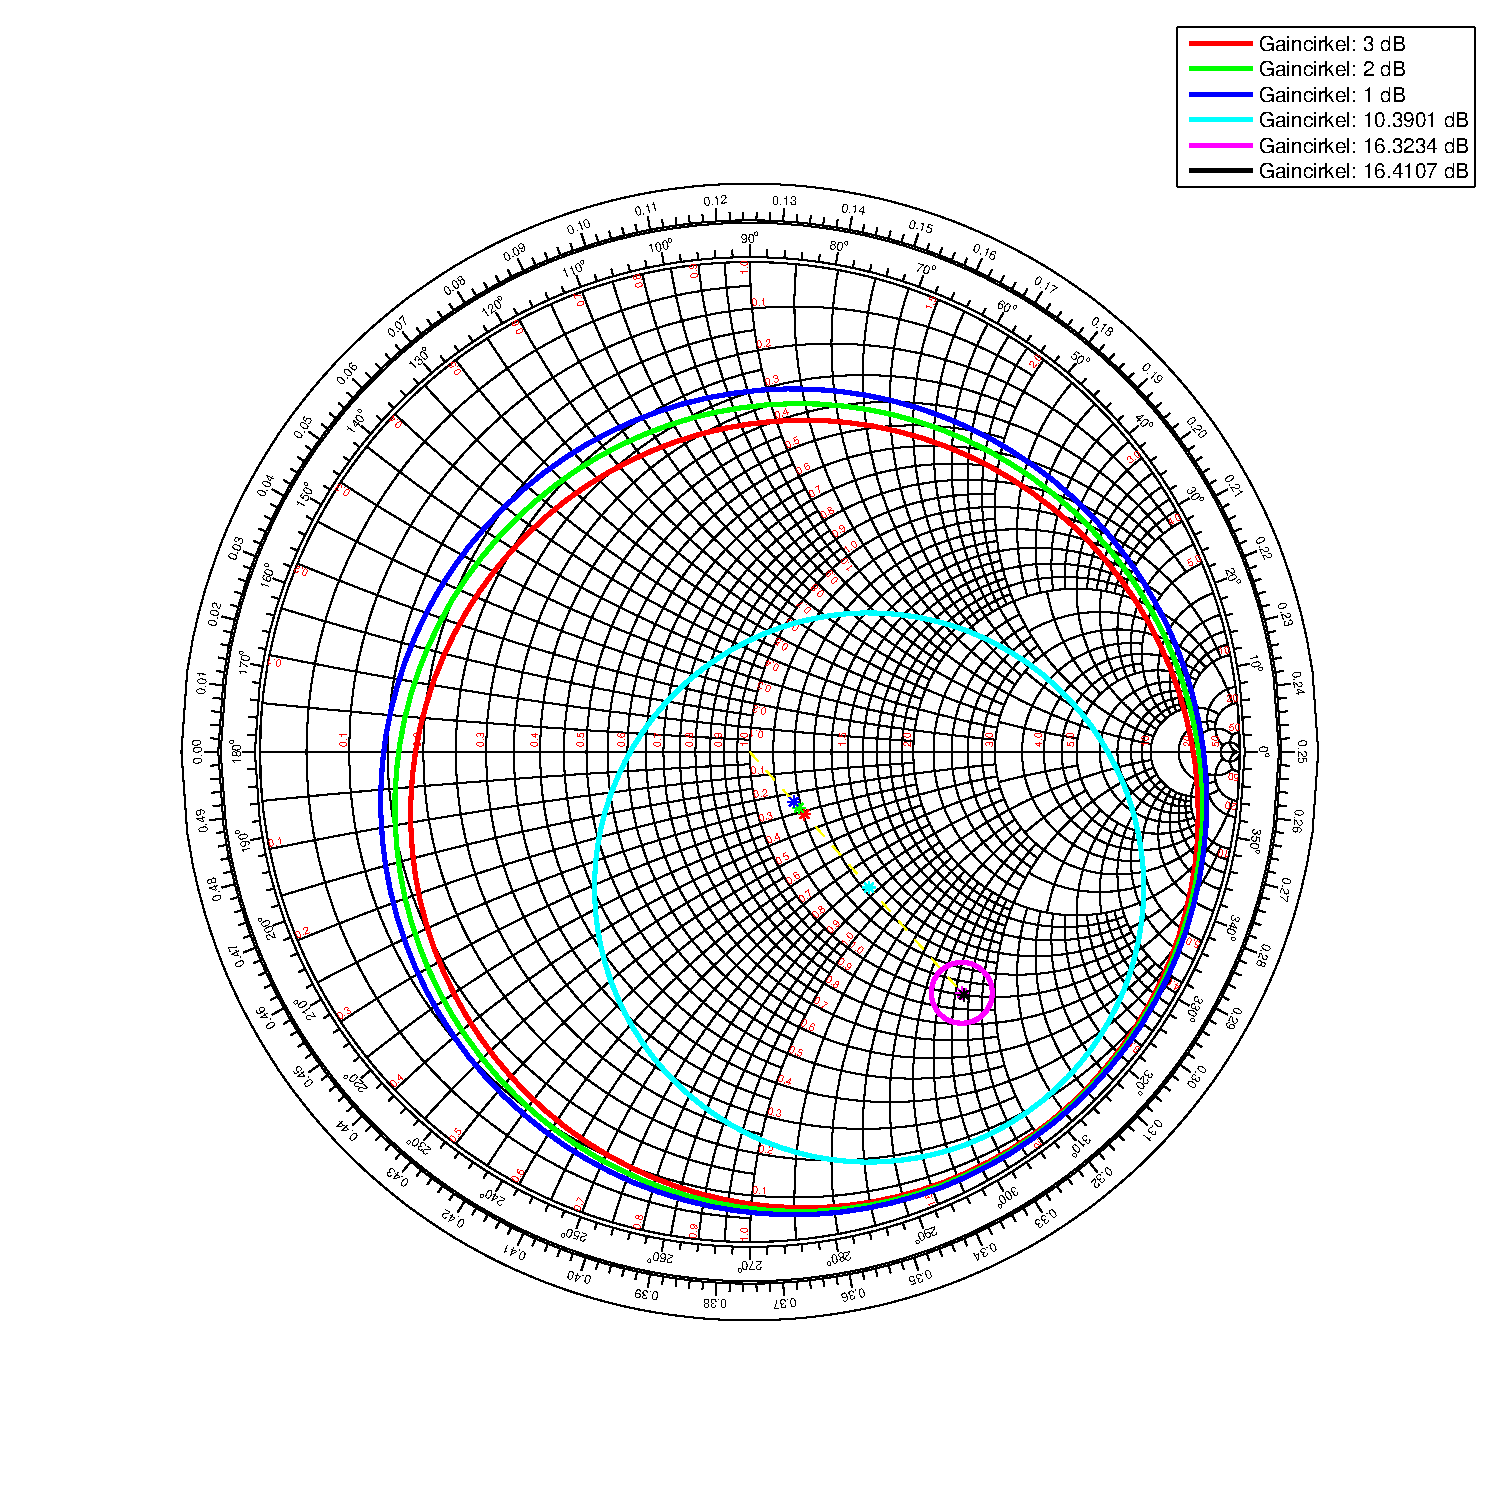
\includegraphics[width=\textwidth,keepaspectratio=true]{fig/gaincirkels.pdf}  
      \caption{Constante gaincirkels} 
      \label{fig:gainCirkels}
    \end{figure}
  

\section{Matchingnetwerken}
  De matching gebeurt zowel voor ingang als uitgang gelijkaardig, vandaar ook
  dat er gekozen is om dit via MATLAB te implementeren in de functie \texttt{matcher}.

  Zoals opgelegd in \cite{lesWendy} wordt gebruikgemaakt van een variatie op de
  single stub matching zoals weergegeven in figuur \ref{fig:schakelingMatch}.

  \begin{figure}[!hb]
    \centering
    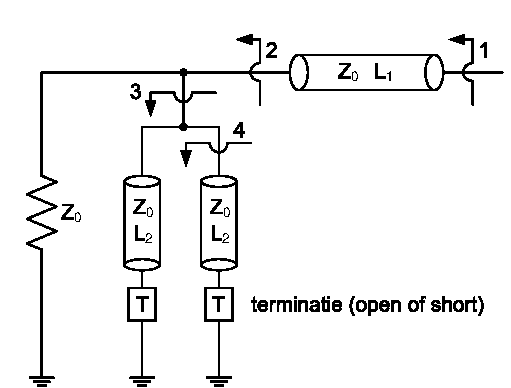
\includegraphics[keepaspectratio=true]{fig/matching.pdf}
    \caption{Schakeling matchingnetwerken}
    \label{fig:schakelingMatch}
  \end{figure}

  \tbd{Procedure invoegen}

  Voor de ingang en uitgang kunnen de bijhorende smith charts op respectievelijk
  figuur \ref{fig:matchIn} en figuur \ref{fig:matchOut} gevolgd worden. Deze zijn
  tevens in de bijlagen aanwezig voor de duidelijkheid.

  \begin{figure}
    \centering
    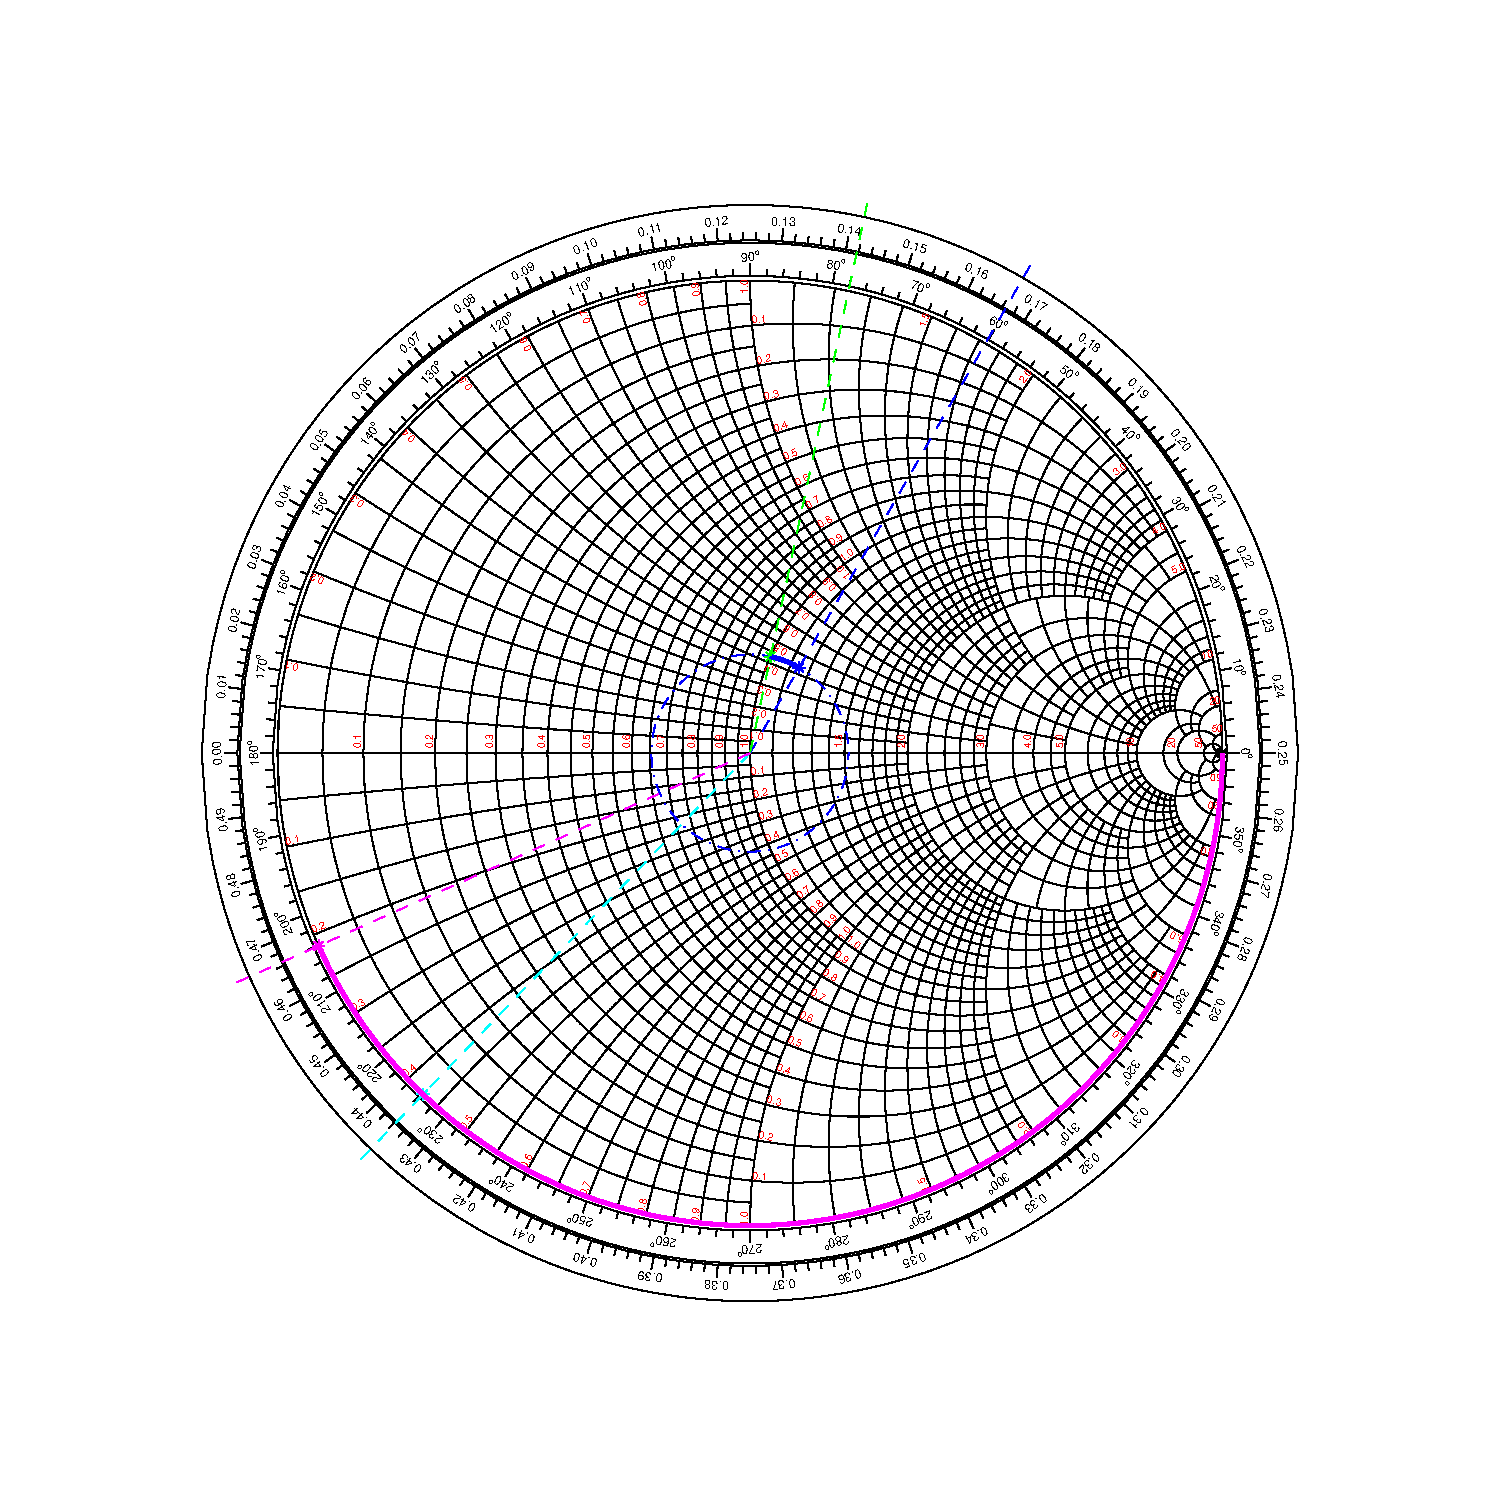
\includegraphics[width=\textwidth,keepaspectratio=true]{fig/matchSource.pdf}
    \caption{Smith Chart matchingnetwerk aan de ingang}
    \label{fig:matchIn}
  \end{figure}

  \begin{figure}
    \centering
    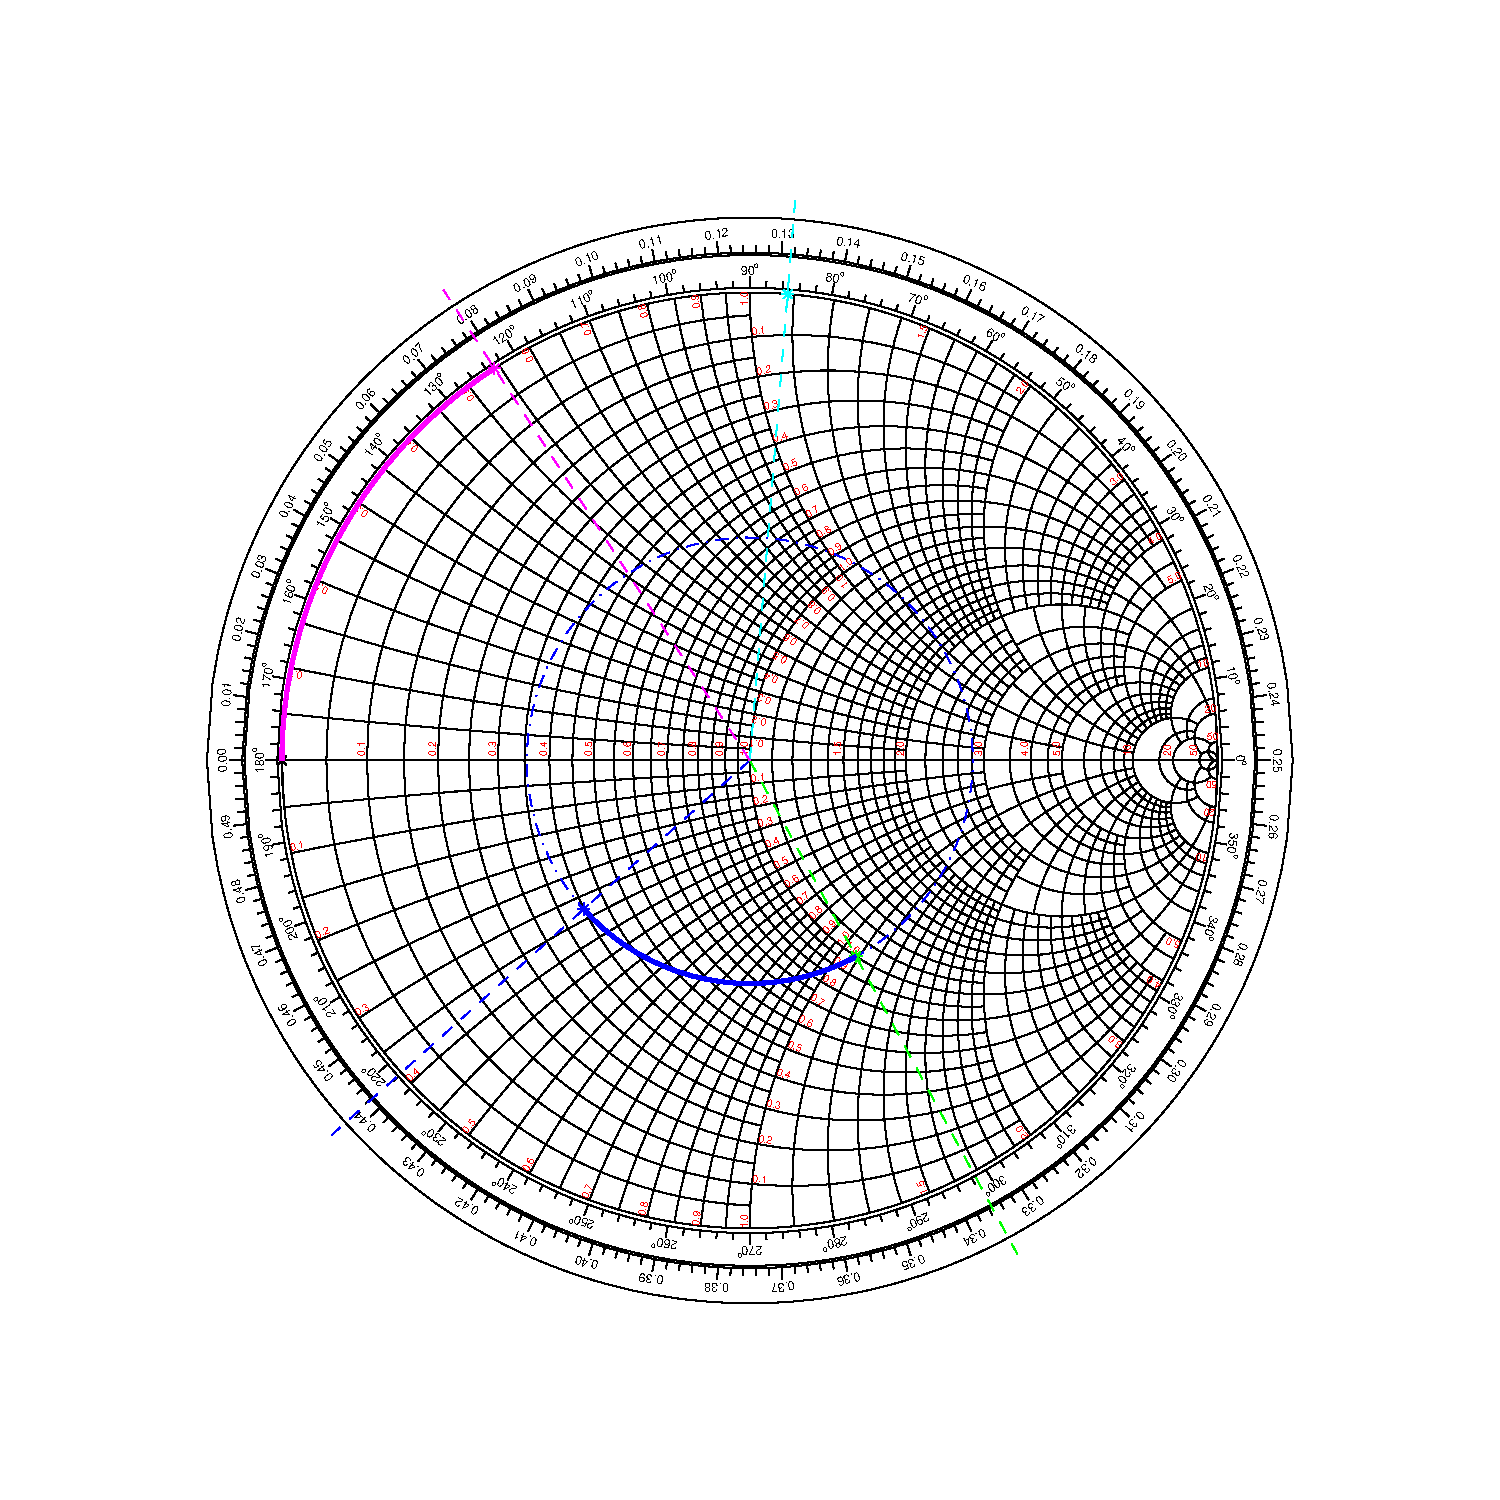
\includegraphics[width=\textwidth,keepaspectratio=true]{fig/matchLoad.pdf}
    \caption{Smith Chart matchingnetwerk aan de uitgang}
    \label{fig:matchOut}
  \end{figure}
  
  De numerieke resultaten van deze matching wordt weergegeven in tabel \ref{tbl:Matching}.

  \begin{table}[h!]
     \begin{center}
       \caption{Matchingnetwerken}
       \label{tbl:Matching}
       \begin{tabular}{|lc|r|r|c|} 
\hline \textbf{Grootheid} & & \textbf{Ingang} & \textbf{Uitgang} & \\ 
\hline $\Gamma_1$ &  & $-0.401 -0.441 j$ & $0.563 +0.448 j$ &  \\ 
\hline $\Gamma_2$ &  & $0.355 -0.479 j$ & $0.517 +0.500 j$ &  \\ 
\hline $Y_2$ &  & $1.000 -1.485 j$ & $1.000 +2.071 j$ & S \\ 
\hline $\Gamma_3$ &  & $0.376 +0.927 j$ & $0.622 -0.783 j$ &  \\ 
\hline $Y_3$ &  & $-1.485 j$ & $+2.071 j$ & S \\ 
\hline $\Gamma_4$ &  & $-0.289 +0.957 j$ & $0.035 -0.999 j$ &  \\ 
\hline $Y_4$ &  & $-0.743 j$ & $+1.035 j$ & S \\ 
\hline $E_1$ &  & 78.896 & 5.500 & $^{\circ}$ \\ 
\hline $E_2$ &  & 73.201 & 88.005 & $^{\circ}$ \\ 
\hline terminatie &  & short & open &  \\ 
\hline \end{tabular} 

     \end{center}
  \end{table}


\section{DC biasnetwerk}
  Om het DC Bias-netwerk te designen kunnen vele verschillende soorten
  netwerken gebruikt worden. Hier werd de aanpak uit \cite{Gonzalez}
  gebruikt. Volgens deze bron is dit netwerk (figuur \ref{fig:DCBias} goed geschikt door
  \begin{itemize}
   \item 
  \end{itemize}

  \begin{figure}
    \centering
    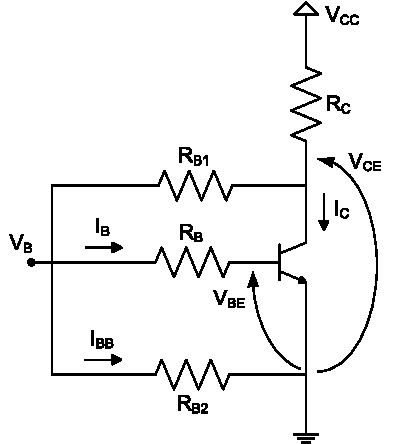
\includegraphics[keepaspectratio=true]{fig/DCBias.pdf}
    \label{fig:DCBias}
    \caption{Biasnetwerk}
  \end{figure}



\section{Simulaties}
  \subsection{Ideale transmissielijnen}
  \subsection{Microstrip}

\section{Lay-out}

\section{Metingen}
\subsection{Vergelijking metingen en simulaties}




\tbd{\textbf{Voor het verslag:}
  \begin{itemize}
    \item Alle berekeningen + verwijzing formule
    \item Plots van ideale simulaties + simulatie in microstripversie
    \item Gebruikte Smith Charts voor matching van in- en uitgang
  \end{itemize}
  }

  \newpage
  \part{Antenne}
  \label{sec:AE}

    % ANTENNE
\section{Dipool}

\section{Balun}

\section{Lay-out}

\section{Metingen}


\tbd{\textbf{Voor het verslag:}
    \begin{itemize}
    \item Alle berekeningen + verwijzing formule
    \end{itemize}
  }
    
  \newpage

  \bibliographystyle{plain}
  \addcontentsline{toc}{section}{Referenties}
  \bibliography{referenties}
  
  
\end{document}